% !TEX root = ../../prj4projektdokumentation.tex

\section{Modultest}

Efter udvikling af Måleenheden er der lavet test på modulet, for at sikre den lever op til  kravene.

\subsection*{Test af spændingsmåling}
\begin{center}
	\begin{tabular}{ | m{0.2\textwidth} | m{0.8\textwidth}|} 
		\hline
		\textbf{Test}					&Spændingsmåling \\ \hline
		\textbf{Testbeskrivelse}		&Der måles ved tre forskellige spændingsniveauer for at sikre at systemet kan måler i hele måleområdet  \\ \hline
		\textbf{Input}					&Test 1: 1,02V. Test 2: 4,02V. Test 3: 8,08V\\ \hline
		\textbf{Forventet output}		&Test 1: 1,02V. Test 2: 4,02V. Test 3: 8,08V\\ \hline
		\textbf{Resultat}				&Test 1: 0,97V. Test 2: 4,00V. Test 3: 8,05V\\ \hline
	\end{tabular}
\end{center}


\subsection*{Test af strømmåling}
\begin{center}
	\begin{tabular}{ | m{0.2\textwidth} | m{0.8\textwidth}|} 
		\hline
		\textbf{Test}					&Strømmåling \\ \hline
		\textbf{Testbeskrivelse}		&Der måles ved 3 forskellige strømniveauer for at sikre at systemet kan måler i hele måleområdet  \\ \hline
		\textbf{Input}							&Test 1: 0,10V. Test 2: 0,30V. Test 3: 0,50V.\\ \hline
		\textbf{Forventet output}		&Test 1: 0,10V. Test 2: 0,30V. Test 3: 0,50V. \\ \hline
		\textbf{Resultat}					&Test 1: 0,10V. Test 2: 0,30. Test 3: 0,50V.\\ \hline
	\end{tabular}
\end{center}


\subsection*{Test af power factor}
\begin{center}
	\begin{tabular}{ | m{0.2\textwidth} | m{0.8\textwidth}|} 
		\hline
		\textbf{Test}					&Power factor måling \\ \hline
		\textbf{Testbeskrivelse}		&Der måles om Power factor stemmer overens med den enlige Power factor. Dette gøres vinklen mellem strøm og spænding på oscilloskop, og derefter regnes power factor.   \\ \hline
		\textbf{Input}					&2 sinus signaler med faseforskydning på 1,9ms svarende til en power factor på 0,827. Se Figur \ref{fig:MaalTest}. \\ \hline
		\textbf{Forventet output}		&Power factor på 0,827\\ \hline
		\textbf{Resultat}				&Power factor på 0,842 \\ \hline
	\end{tabular}
\end{center}   

\begin{figure}[H] % (alternativt [H])
	\centering
	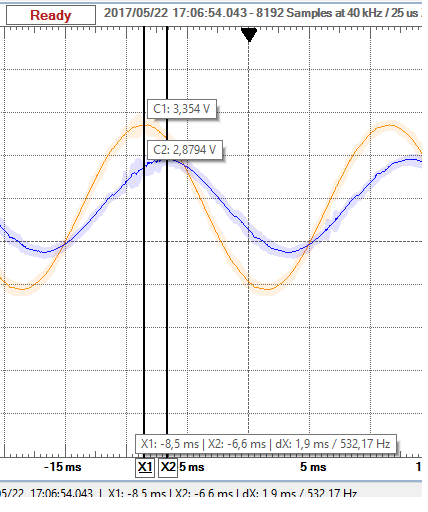
\includegraphics[width=0.5\textwidth]{Figure/MaalTest}
	\caption{Sinussignaler med faseforskydning anvendt til test af power factor.}
	\label{fig:MaalTest}
\end{figure}


\subsection*{Test af THD måling}
Test af THD kan ses i kapitel \ref{sek:THD}. 